One of the usual questions regarding smooth manifolds is the existence of topological invariants. In particular, one often wants to know which properties of a manifold depend only on the underlying topology.

For instance, the De Rham cohomology measures the obstruction to the integrability of closed forms in a manifold. This means, for $\alpha \in \Omega^k(M)$ with $d\alpha = 0$, to what extent the equation
\[d\beta = \alpha\]
is not solvable.

Morse theory constructs a topological invariant based on the critical points of certain (regular enough, as we will explain later) smooth functions $f : M \rightarrow \R$. As a starting example, we may think of a torus, vertically embedded inside $\R^3$, as shown in Figure \ref{figure:torus}.

\begin{figure}[h]
	\centering
	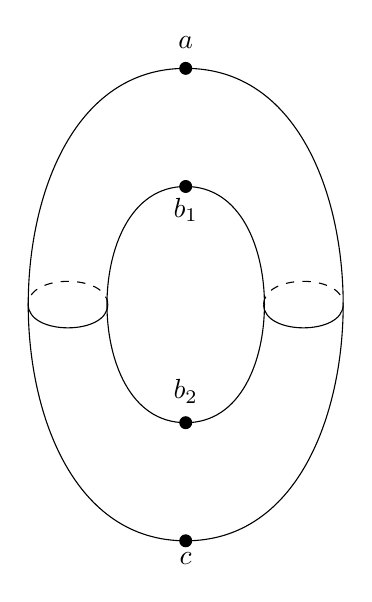
\begin{tikzpicture}
	%Draw the torus
	\draw [] (0,3) to [out=0,in=90] (2,0) to [out=270,in=0] (0,-3) to [out=180,in=270] (-2,0) to [out=90,in=180] (0,3);
	\draw [] (1,0) to [out=270,in=0] (0,-1.5) to [out=180,in=270] (-1,0) to [out=90,in=180] (0,1.5) to [out=0,in=90] (1,0);
	\draw [] (-2,0) to [out=270,in=270] (-0.99,0);
	\draw [dashed] (-0.99,0) to [out=90,in=90] (-2,0);
	\draw [] (2,0) to [out=270,in=270] (0.99,0);
	\draw [dashed] (0.99,0) to [out=90,in=90] (2,0);

	%Critical point a
	\draw [fill] (0,3) circle [radius=0.75mm]
	node [label={[above]$a$}] {};
	%Critical point b_1
	\draw [fill] (0,1.5) circle [radius=0.75mm]
	node [label={[below,yshift=-1.5mm]$b_1$}] {};
	%Critical point b_2
	\draw [fill] (0,-1.5) circle [radius=0.75mm]
	node [label={[above]$b_2$}] {};
	%Critical point c
	\draw [fill] (0,-3) circle [radius=0.75mm]
	node [label={[below,yshift=-1.5mm]$c$}] {};
\end{tikzpicture}

	\caption{The torus embedded in $\R^3$.}
	\label{figure:torus}
\end{figure}

The points marked in the figure are the critical points of a function defined on the torus, namely the height function. It is worth, however, not to think of them as critical points yet. Rather, imagine that the torus is fixed in a space that is gradually flooded by water. Let us imagine that the water level is rising, so it covers first the point $c$, then $b_2$, then $b_1$ and finally $a$. Let us think about how the topology of the part of the torus that is submerged in water changes over time:

\begin{itemize}
	\item Before reaching the point $c$ there is no part of the torus under the water level.
	\item After the water crosses the point $c$, the region underwater is homeomorphic to a disk. In particular, it is a contractible space.
	\item Between the points $c$ and $b_2$, the topology of the torus does not change.
	\item After the water passes through the point $b_2$, the topology becomes more interesting. The region under the water looks like a disk to which we have added a strip of the torus: it is homotopic to a disk with a $1$ dimensional cell attached. Another way to see it is that it is homeomorphic to an open cylinder.
	\item After the water covers the point $b_1$, we have added another strip to the manifold. The resulting space is homotopic to the cylinder of the last step with a $1$ dimensional cell attached to it.
	\item After the water covers the point $a$ the whole torus is underwater, so we have recovered the whole manifold. Specificaly, what we add from the last step is a disk, this means, a $2$ dimensional cell.
\end{itemize}

In this examplewe have constructed a cell skeleton of $\con{T}^2$ using the intuition of the water rising. Nonetheless, this intuition can be formalized, as we stated earlier, by studying the critical points of the height function restricted to the torus. From this formalization, we can retrieve the homology of $\con{T}^2$, which is
\[H_k(\con{T}^2) = \left\{ \begin{array}{lc} \con{Z}_2 & \text{if } k=0 \text{ or } 2 \\ \con{Z}_2^2 & \text{if } k=1 \\ 0 & \text{otherwise.} \end{array} \right.\]

We can see that this homology coincides with the cellular homology of the manifold (in fact, this is always the case).

Morse theory, then, relates the topology of the manifold with the critical points of a function defined over it. The truly unexpected result about this relationship is that it does not depend on the particular function that we are choosing to define the complex: the resulting homology is invariant. In consequence, we get some information on the number of critical points of any function over the manifold (assuming that it satisfies some regularity condition). In particular, the most remarkable result are the Morse inequalities, that yield a lower bound for the number of critical points.

The main focus of this master thesis is not to understand what is the Morse homology, but rather to see how it is constructed, this means, what are the steps that one has to take to define it. We do it this way because these steps are the unifying thread with the second part of the thesis, namely Floer homology.

Floer homology was developed by Andreas Floer in the middle 80's in order to prove the Arnold conjecture. This conjecture states that there is a number of periodic orbits of a Hamiltonian system under certain conditions, and is both interesting from the point of view of symplectic geometry and the study of dynamical systems.

The insight that Floer provided was that all the ideas that allow us to define the Morse homology can be applied in a different (infinite dimensional) context to construct a homology that studies the $1$-periodic orbits of Hamiltonian systems defined over the manifold. Moreover, as it was the case with Morse homology, this construction depends only on the topology of the underlying manifold and not on the structure required to retrieve the particular periodic orbits, this means, it is a topological invariant. This leads to the interesting conclusion that the (Hamiltonian) dynamics that can be defined over a manifold are constrained by its topology.

This master thesis starts with a complete description of Morse theory in Chapter 1. After that, we talk about symplectic geometry and the Arnold conjecture in more detail in Chapter 2, in order to give the motivation for the study of the Floer homology. In Chapter 3 we present the basic constructions of the theory, focusing on the Floer equation. Finally, we give the ideas of how the Arnold conjecture is proved, and talk about some other results that can be proved with the tools that we provide in this thesis.
